\documentclass[12pt,oneside]{memoir} 

\usepackage[latinica,biblatex]{matfmaster} 
\usepackage{tabu}
\usepackage{graphicx}
\graphicspath{ {./images/} }
\usepackage{listings}
\renewcommand{\lstlistingname}{Primer koda}% Listing -> Primer koda
\lstset{language=C++,
	basicstyle=\ttfamily\scriptsize,
	keywordstyle=\color{blue}\ttfamily,
	stringstyle=\color{red}\ttfamily,
	commentstyle=\color{green}\ttfamily,
	breaklines=true
}

\bib{maturski}

\autor{Lazar Premović}
\naslov{Čovek-mašina interfejs za primenu u muzici}
\podnaslov{Professional Hardware Interfaces - Generic Professional Controller		\textbf{"PHI - GPC"}}
\predmet{Napredne tehnike programiranja}
\godina{maj 2019}
\mentor{Prof. dr Filip Marić}
\apstr{%
	Upravljanje računarom uz pomoć miša i tastature je sasvim dovojno za prosečne korisnike ali za većinu profesionalnih korisnika (pogotovo u Audio/Video oblasti) miš i tastatura nisu optimalan način upravljanja računarom.
	Zato se za većinu profesionalnih primena, na račuare povezuju posebno dizajnirani kontroleri koji olakšavaju i ubrzavaju zadatke koje treba obaviti.
	Međutim kontroleri pored visokih cena imaju još nekoliko ograničenja koji ih čine nepraktičnim: dizajnirani su za određenu vrstu posla (npr. teško je obrađivati slike na kontroleru dizajniranom za miksovanje zvuka) i često rade sa samo jednim programom i vrlo je teško ili nemoguće koristiti ih za upravljane nekim drugim programom.
	\newline
	Zato je cilj ovog rada izrada kontrolera koji je primenjljiv u širokom spektru poslova i moguće ga je povezati sa bilo kojim programom. Da bi se taj cilj ostvario, hardver kontrolera mora biti opšte koncipiran\footnote{Ne specijalizovan ni za jednu konkretnu primenu.} da bi mogao da se primeni na bilo koju vrstu softvera kojim treba da se upravlja, a softver za konfigurisanje mora da omogući veoma detaljnu konfiguraciju kontrolera i lako proširivanje funkcionalnosti.
	\newline
	Tako su nastali:
	\begin{itemize}
		\item \textbf{GPC} \textit{"Generic Professional Controller"} (Kontroler),
		\item \textbf{PHI Control Center}\footnote{Professional Hardware Interfaces Control Center.} (Softver za konfigurisanje i obradu u realnom vremenu),
		\item \textbf{GHP} \textit{"Generic HID\footnote{Human Interface Device} Protocol".} (Protokol za komunikaciju između kontrolera i softvera).
	\end{itemize}
}


\begin{document}

	\frontmatter

	\naslovna

	\apstrakt
	\tableofcontents*

	\mainmatter

	\chapter{Korišćene tehnologije}
	
	\section{Arduino}
	Arduino je projekat otvorenog koda koji dizajnira i proizvodi mikrokontrolere bazirane na \textit{Atmel} 8-bitnim AVR mikrokontrolerima čije se sve neophodne komponente nalaze na jednoj štampanoj ploči.
	Arduino mikrokontroleri se programiraju pomoću Arduino IDE-a\footnote{Integrated Development Environment - Integrisano razvojno okruženje.} koristeći programski jezik C++ i nekoliko dodatnih biblioteka. U kodu je umesto \textit{main()} funkcije neophodno imati funkcije: \textit{setup()} koja se ivzrši samo jednom čim se mikrokontroler uključi i \textit{loop()} koja se poziva dokle god je mikrokontroler uključen. Arduino IDE takođe omogućava prevođenje koda i njegovo učitavanje na mikrokontroler pomoću samo jednog klika čime time olakšava i ubrzava razvoj softvera za Arduino mikrokontrolere. Digitalni pinovi mogu biti u samo dva stanja: logički 1\footnote{Odgovara naponu od 5V} i logički 0\footnote{Odgovara naponu od 0V} u daljem tekstu ćemo ih zvati HIGH i LOW.
	\paragraph{PWM}\label{PWM}
	Pulse Width Modulation, je tehnika kojom je moguće aproksimirati bilo koji izlazni napon čak iako pin može biti samo u HIGH ili LOW stanju. To se postiže tako što pin vrlo brzo menja stanja a podešavanjem odnosa vremena kada je pin HIGH i LOW moguće je tačno precizirati traženi napon. 
	\section{C\# desktop aplikacije}
	C\# je programski jezik opšte namene koji je razvio Microsoft za potrebe razvojnog okruženja \textbf{.NET Framework}. C\# podržava objektno orjentisanu, imperativnu, deklarativnu i generičku programsku paradigmu. Deo C\#-a je i paket \textbf{Windows Forms} koji omogućava brzo i lako kreiranje desktop aplikacija sa grafičkim interfejsom uz pomoć Microsoft Visual Studio IDE-a.
	\section{JSON}
	JavaScript Object Notation \textbf{JSON} je format za čuvanje i prenos podataka u kome su podaci zabeleženi tako da ih je vrlo lako učitati i prevesti u odgovarajući objekat. Svaki zabeleženi podatak je predstavljen kao par ključa i vrednosti. Tipovi podataka koje JSON podržava su: string,int,bool,null,niz i objekat (koji može sadržati bilo koji tip).
	\section{MIDI}
	Musical Instrument Digital Interface \textbf{MIDI} je standard koji opisuje komunikacioni protokol, digitalni interfejs i fiziče konektore koji omogućuju povezivanje raznovrsnih digitalnih audio uređaja. MIDI protokol definiše MIDI poruke koje su sačinjene od statusnog bajta i do dva bajta sa podacima koji se prenose serijski brzinom od 31.25 kbit\textbackslash s. Statusni bajtovi su uvek $\geq$128 dok su bajtovi sa podacima <128. MIDI definiše nekoliko statusnih bajtova kao što su NoteOn (nota je pritisnuta), NoteOff (nota je otpuštena) i ControlChange (vrednost kontrole se promenila), koji je bitan zato što se uglavnom koristi za komunikaciju kontrolera i audio softvera. MIDI definiše da posle ControlChange statusnog bajta slede dva bajta: prvi bajt sadrži ID kontrole iz opsega 0-127 i drugi bajt koji sadrži novu poziciju kontrole iz opsega 0-127.
	\subsection{virtualMIDI}
	Kako MIDI standard definiše samo komunikaciju između dva hardverska uređaja ili između hardvera i softvera. Da bi ostvarili komunikaciju između dva softvera (u ovom slučaju odabranog audio softvera i \textbf{PHI Control Center}-a koji služi kao posrednik između audio softvera i kontrolera) koristimo biblioteku koja nam omogućava kreiranje virtuelnog MIDI uređaj i njegovo korišćenje za slanje MIDI poruka.
	virutalMIDI Tobias Erichsen-a je biblioteka koja nam to omogućava. Za njeno korišćenje potrebno je instalirati loopMIDI ili rtpMIDI softver, uz koji dolazi drajver za koji se virtualMIDI povezuje. Nakon toga je dovoljno uključiti .cs fajl biblioteke u projekat i koristiti metode za kreiranje virtuelnog uređaja i slanje poruka preko njega.
	\chapter{GHP Protokol}
	Da bi kontroler mogao da komunicira sa softverom za konfiguraciju osmišljen je i definisan protokol koji će se koristiti.
	GHP kao svoju osnovu koristi serijsku komunikaciju preko USB-a sa podešenim baud rate-om\footnote{Brzina prenosa podataka, u digitalnoj komunikaciji ekvivalentna sa brojem bitova u sekundi.} od 115200\footnote{115.2 kbit\textbackslash s.}.Poruke koje se šalju ovim protokolom imaju sledeći format:\newline
	\centerline{\textit{CommandByte, ChannelByte, $\left[0-20\right]$DataBytes}.}\newline
	\textbf{Komandni bajt} govori o kojoj komandi je reč i takođe time precizira broj bajtova sa podacima koji će uslediti (za spisak komandi pogledati tabelu \ref{Tabela:1}). Radi lakšeg razumevanja sve vrednosti komandnih bajtova su iz alfanumeričkog opsega ASCII enkodiranja tako da ih možemo lakše obeležavati po ASCII karakteru koji im odgovara. \newline
	\textbf{Bajt koji označava kanal} govori na koju kontrolu ili memorijsku adresu se odnosi komanda.\newline
	\textbf{Bajtovi sa podacima} sadrže podatke karakteristične za određenu komandu.\newline
	\begin{table}[h]
		\begin{tabu} to 1\textwidth { | X[c] | X[c] | X[c] | X[c] | }
		\hline
		Komandni bajt & Komanda & Kanal & Opis bajtova sa podacima \\
		\hline
		'B' \textit{66} & Taster je pritisnut & Indeks tastera & NEMA  \\
		\hline
		'R' \textit{82} & Taster je otpušten & Indeks tastera & NEMA  \\
		\hline
		'A' \textit{65} & Analogna kontrola je pomerena & Indeks analogne kontrole & 2 bajta. Nova vrednost analogne kontrole, Little Endian enkodiranje \\
		\hline
		'I' \textit{73} & Rotacioni enkoder je inkrementovan & Indeks enkodera & NEMA  \\
		\hline
		'D' \textit{68} & Rotacioni enkoder je dekrementovan & Indeks enkodera & NEMA  \\
		\hline
		'L' \textit{76} & Podesi LED & Indeks diode & 3 bajta. \textit{R, G, B}  \\
		\hline
		'l' \textit{108} & Podesi LCD & Broj linije ekrana & 20 bajtova. Tekst  \\
		\hline
		'P' \textit{80} & Podesi trajni podatak & Memorijska adresa & 1 bajt. \textit{Vrednost}  \\
		\hline
		'p' \textit{112} & Zahtev za vrednost trajnog podatka & Memorijska adresa & NEMA  \\
		\hline
		'r' \textit{114} & Odgovor na zahtevanu vrednost & Memorijska adresa & 1 bajt. \textit{Vrednost}  \\
		\hline
		'S' \textit{83} & Sistemska komanda (videti tabelu \ref{Tabela:2}) & Vrsta sistemske komande & Zavisi od vrste sistemske komande  \\
		\hline
		\end{tabu}
		\caption{Objašnjenje komandnih bitova}
		\label{Tabela:1}
	\end{table}
	\begin{table}[h]
	\begin{tabu} to 1\textwidth { | X[c] | X[c] | X[c] | }
		\hline
		Vrsta sistemske komande & Komanda & Opis bajtova sa podacima \\
		\hline
		'W' \textit{87} & Zahtev za indentifikacioni broj uređaja &  NEMA  \\
		\hline
		'w' \textit{119} & Odgovor na zahtev za indentifikacioni broj uređaja & 1 bajt. \textit{Identifikacioni broj uređaja} \\
		\hline
		'R' \textit{82} & Resetuj uređaj & NEMA \\
		\hline
	\end{tabu}
	\caption{Objašnjenje sistemskih komandi}
	\label{Tabela:2}
\end{table}
	\chapter{Kontroler}
	
	\begin{figure}[h]
		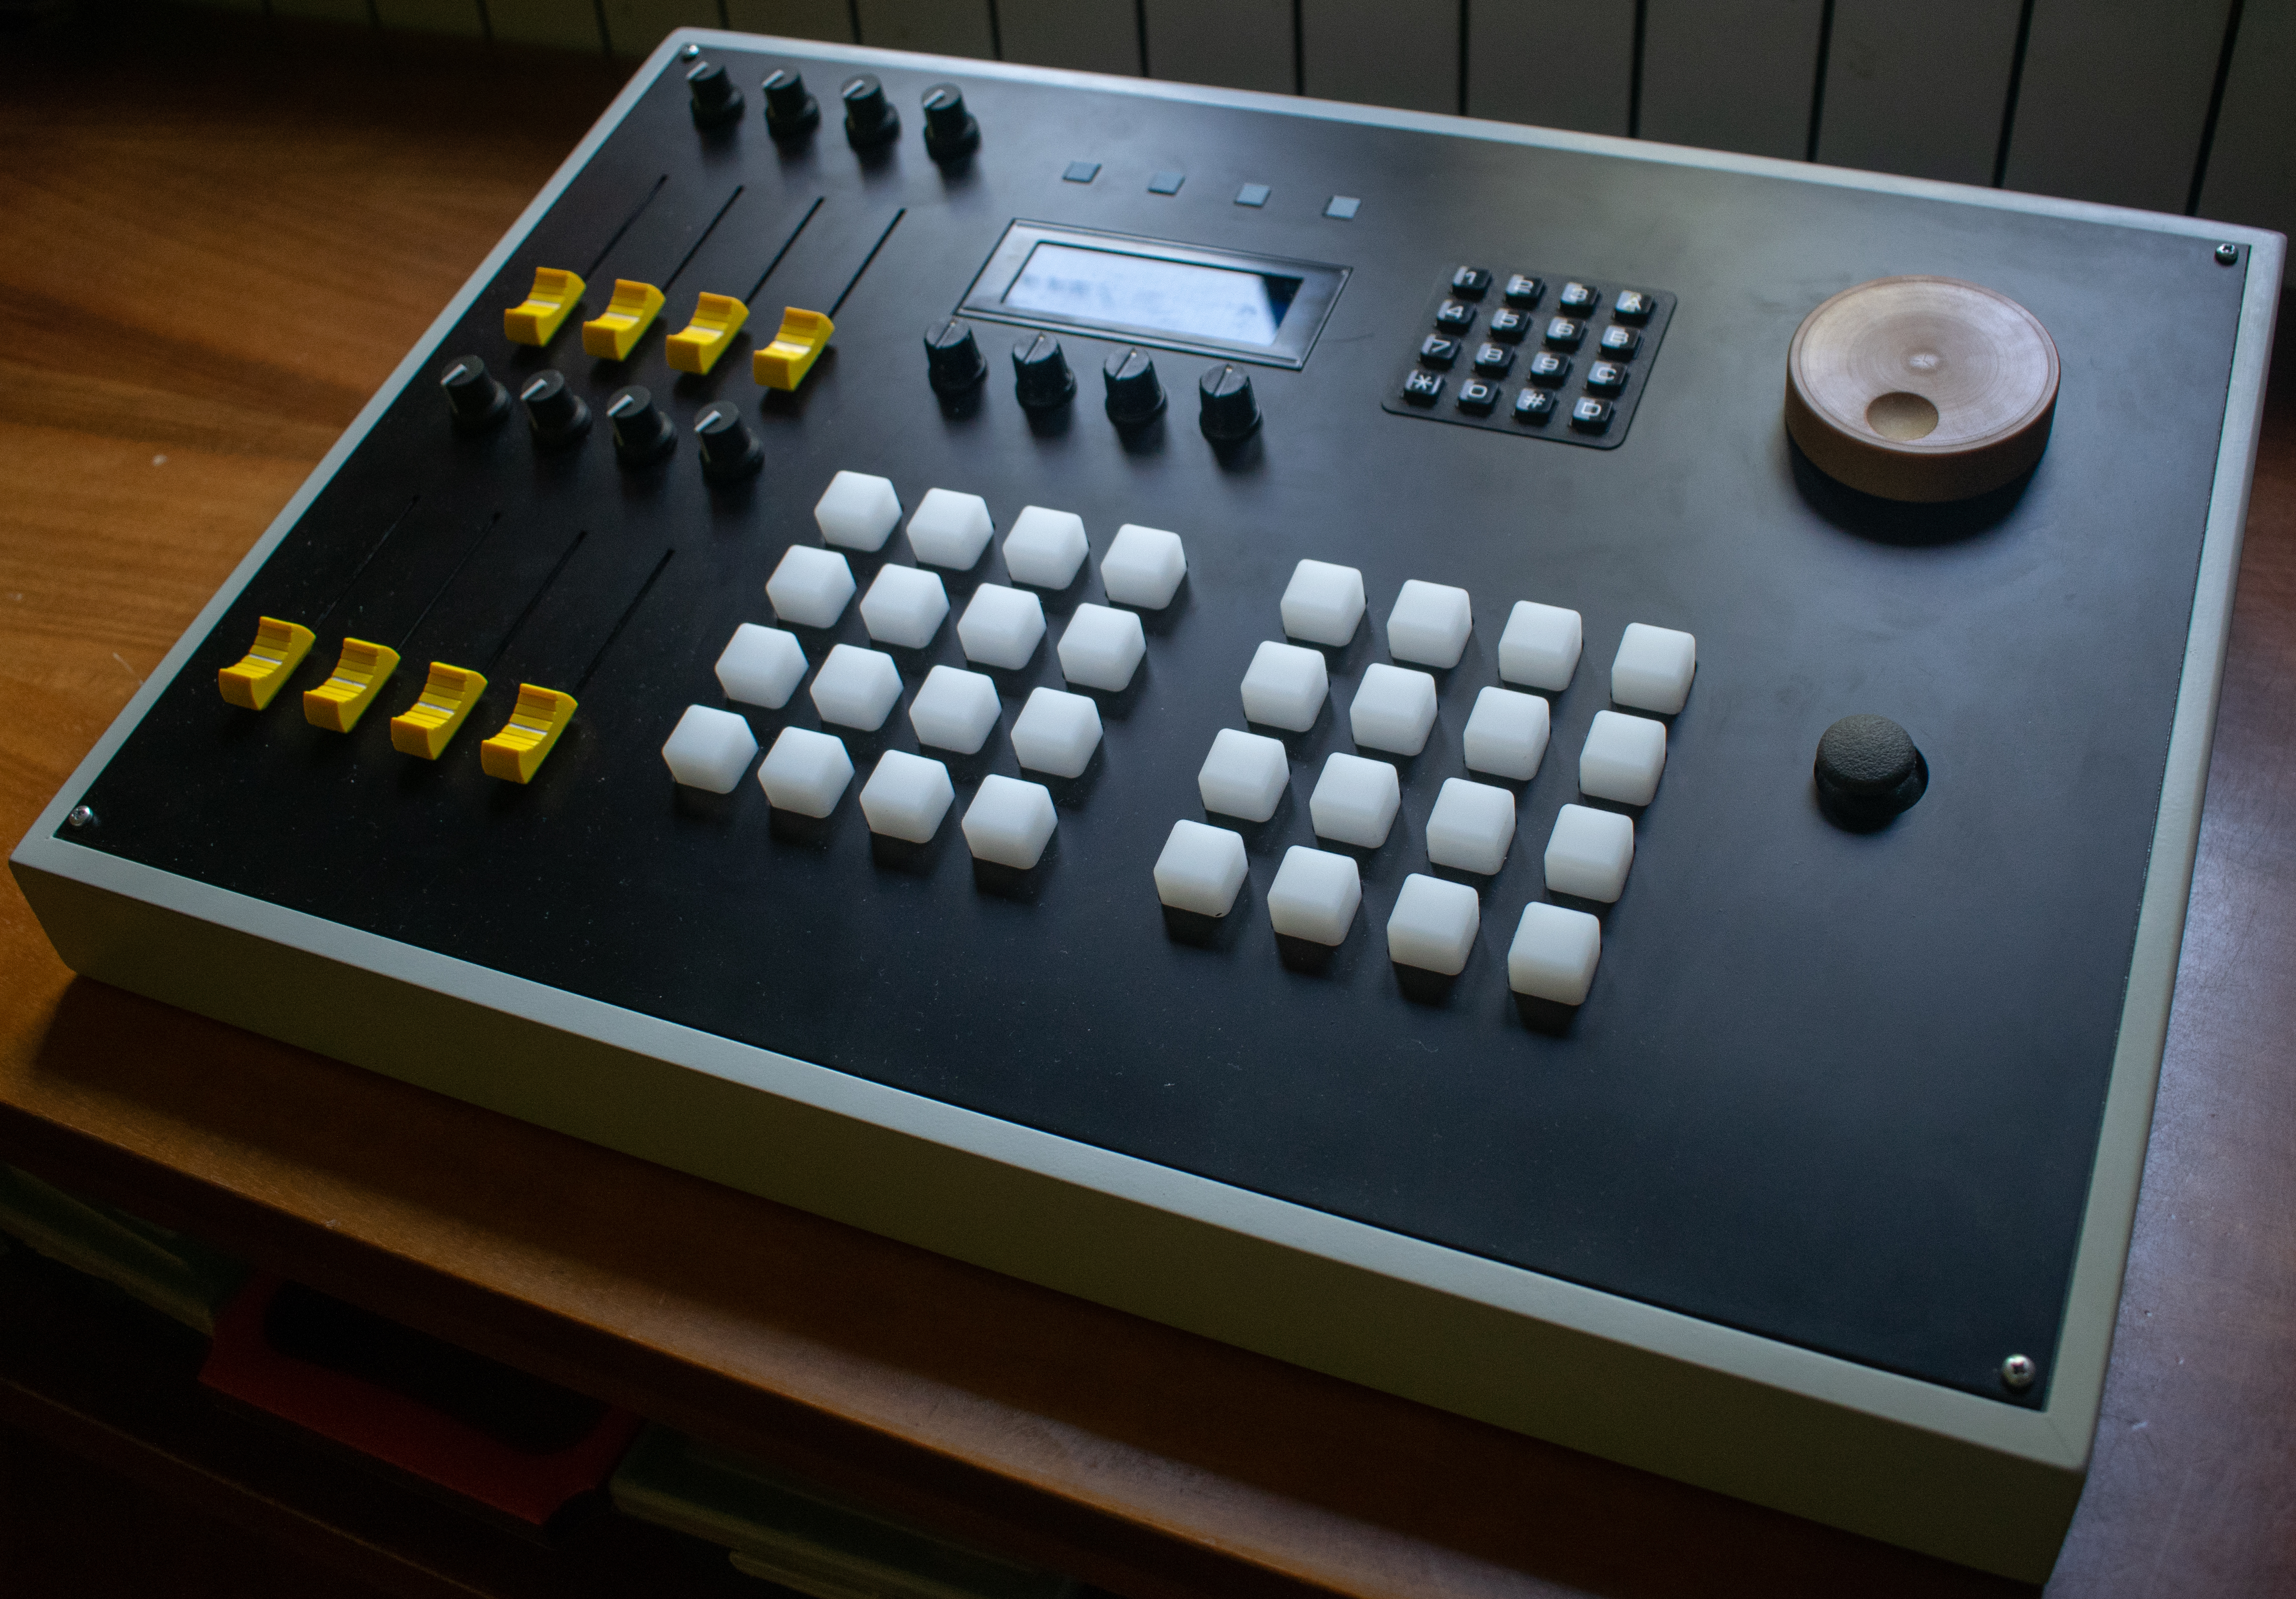
\includegraphics[width=\textwidth]{GPC}
		\caption{GPC kontroler}
		\label{Slika:GPC}
	\end{figure}
	
	Funkcija kontrolera je da akcije korisnika prenese softveru za obradu u realnom vremenu.
	Taj proces zahteva sledeće korake:
	\begin{enumerate}
		\item učitavanje stanja kontrola,
		\item detekciju promena stanja kontrola,
		\item slanje informacija o promeni stanja kontrola koristeći GHP protokol,
		\item ažuriranje stanja displeja i dioda na osnovu informacija primljenih GHP protokolom.
	\end{enumerate}
	Zato GPC ima nekoliko integralnih kola koja pomažu pri učitavanju stanja kontrola i Arduino Mega mikrokontoler koji vrši sve ostale operacije i implementira GHP protokol.
	\paragraph{Karakteristike Arduino Mega mikrokontrolera}
	\begin{itemize}
		\item ATmega2560 mikrokontroler
		\item 54 Digitalna ulazno/izlazna pina (od kojih 15 imaju podršku za PWM\footnote{Pogledati \ref{PWM}.})
		\item 16 Analognih ulaznih pinova
		\item 256 KB Programske memorije
		\item 8 KB RAM memorije
		\item 4 KB EEPROM\footnote{Electrically Erasable Programmable Read-Only Memory.} stalne memorije
	\end{itemize}
	\section{Hardver}
	\subsection{Kontrolna površina}
	\begin{figure}[h]
		\includegraphics[width=\textwidth]{Top}
		\caption{Kontrolna površina}
		\label{Slika:Top}
	\end{figure}
	
	Kontrolnu površinu čine nekoliko disjunktnih grupa (videti sliku \ref{Slika:Top}).
	\begin{itemize}
		\item Analogna sekcija (krajnje levo) sadrži 8 kliznih i 8 rotacionih potenciometara koji u zavisnosti od svoje pozicije mogu imati vrednosti u opsegu 0-1023
		\item Sekcija sa tasterima (dve matrice sa belim tasterima i numerička tastatura) sadrži 48 tastera podeljena u tri 4x4 matrice (donja leva matrica takođe sadrži RGB LED diode ispod svakog tastera) i šalje informaciju kada se neki od tastera pritisne ili otpusti.
		\item Displej i prateće kontole, ispod displeja se nalaze 4 beskonačna rotaciona enkodera koji šalju informaciju kada su inkrementovani\footnote{Okrenuti za jedan stepen u smeru kazaljke na satu.} ili dekrementovani\footnote{Okrenuti za jedan stepen u smeru suprotnom od kazaljke na satu.} a iznad se nalaze 4 tastera i svi su namenjeni da izvršavaju funkcije prikazane na displeju.
		\item Točak za brzu navigaciju (Jog wheel) i džojstik su zasebni elementi. Točak se realizuje pomoću rotacionog enkodera, a džojstik kao spoj dve analogne kontrole za x i y ose i tastera koji reaguje kada se džojstik pritisne. 
	\end{itemize}
	
	\section{Elektronika i integrisana kola}	
	Da bi se gore navedene kontrole povezale potrebno je: $$16+48+3*16\footnote{Po tri za svaku LED diodu.}+4+2*5\footnote{Po dva za svaki enkoder}+6\footnote{Za displej.}+3=135$$ pinova, mnogo više nego što mikrokontroler ima, zato je neophodno upotrebiti nekoliko tehnika kojima se taj broj smanjuje na manje od $\approx$70.
	\paragraph{Matrice tastera}
	Matrice tastera nam omogućavaju da $N$ tastera povežemo koristeći samo $2\sqrt{N}$ pinova tako što tastere rasporedimo u matricu. Čitanje vršimo tako što po jednu kolonu postavljamo HIGH i onda čitamo vrednosti redova. Ono što poboljšava ovo rešenje je da sve ulazne\footnote{pinove na kolonama.} pinove svih matrica spojimo i efektivno dobijemo jednu veliku $\sqrt{N}\times3\sqrt{N}$ matricu koja koristi samo $4\sqrt{N}$ pinova za $3N$ tastera. Sličan princip može se primeniti i na LED diode, time se dobijaju tri matrice (po jedna za svaku boju) koje se opet mogu spojiti u $\sqrt{N}\times3\sqrt{N}$ matricu.
	Ovim je broj potrebnih pinova smanjen na: na:$$16+16\footnote{$\sqrt{N}\times3\sqrt{N}$ matrica tastera.}+16\footnote{$\sqrt{N}\times3\sqrt{N}$ matrica LED dioda.}+4+2*5+6+3=71$$ što je još uvek više od broja slobodnih pinova na mikrokontroleru.
	\paragraph{Multipleksiranje}
	Multipleksiranje nam omogućava da korsiteći specijalno integrisano kolo smanjimo broj potrebnih pinova sa $N$ na $(\log_{2}N)+1$. To postižemo tako što svaki ulaz adresiramo po binarnoj reprezentaciji njegovog indeksa a broj bitova u binarnoj reprezentaciji nekog broja je $\log_{2}N$ i još jedan pin za čitanje izabranog ulaza čime dobijamo $(\log_{2}N)+1$. U ovom projektu su koriščena dva tipa multipleksera: multiplekser sa 8 ulaza (koristi samo 4 pina) i multiplekser sa 4 ulaza (koristi samo 3 pina). Sledeća optimizacija koju možemo da izvršimo jeste da pinove za selekciju svih multipleksera istog tipa povežemo zajedno i time dobijamo $N*M\footnote{N broj ulaza multipleksera, M broj multipleksera.}$ ulaza sa samo $(\log_{2}N)+M$ pinova. U kontroleru se nalaze 4 multipleksera sa 8 ulaza i 3 multipleksera sa 4 ulaza. Dva multipleksera sa 8 ulaza se koriste za ulaze iz analogne sekcije dok druga dva pokrivaju izlaze iz matrice tastera i tastere iznad displeja. Svaki od multipleksera sa 4 kanala je zadužen za ulaze po jedne matrice LED dioda (po jedna matrica za svaku boju).Trenutni broj potrebnih pinova je: $$3\footnote{Selektori za multipleksere sa 8 kanala.}+4\footnote{Ulazi za multipleksere sa 8 kanala.}+2\footnote{Selektori za multipleksere sa 4 kanala.}+3\footnote{Izlazi za multipleksere sa 4 kanala.}+4\footnote{Izlazi za matricu tastera.}+4\footnote{Izlazi za matricu LED dioda.}+2*5+6+3=39$$ što je dovoljno mali broj da se poveže na mikrokontroler.
	\newline
	Za šemu elektronike pogledajte sliku \ref{Slika:schem}, a detaljnije šeme i tehnički crteži se nalaze na priloženom CD-u.
	\section{Mikrokontrolerski kod}
	Kod koji se izvršava na mikrokontroleru se sastoji od glavnog fajla koji sadrži funkcije \textit{setup()} i \textit{loop()} i još nekoliko biblioteka koje sam napisao\footnote{Sve biblioteke su sačinjene od istoimenih .cpp i .h fajlova.}, a to su:
	\begin{itemize}
		\item \textbf{define} biblioteka koja sadrži sve konstante (npr. brojeve pinova) i globalne promenljive koje su potrebne,
		\item \textbf{lib} biblioteka koja sadrži neke funkcije koje mogu biti korisne i u drugim projektima (upravljanje matricama tastera, multiplekserima i opreacije nad nizovima pinova),
		\item \textbf{GHP} biblioteka koja implementira GHP protokol za komunikaciju sa računarom,
		\item \textbf{Peristence} biblioteka koja olakšava trajno skladištenje i čitanje podataka.
	\end{itemize}
	\subsection{Čitanje tastera}
	\label{bounce}
	Ukoliko su tasteri lošeg kvaliteta ili se ne pritisnu u potpunosti, može doći do odskakivanja kontakata unutar tastera što se može registrovati kao više pritisaka umesto samo jednog. Zato je na svim tasterima kontrolera implementrian \textit{Debouncing\footnote{Algoritam za uklanjanje odskakivanja.}} algoritam.
	\begin{lstlisting}[language=C++]
byte val=digitalRead(MUXDR[0]);
if(val==HIGH && ButtonDebounce[ind]<DEBOUNCE)
{
  ButtonDebounce[ind]++;
  if(ButtonDebounce[ind]==DEBOUNCE && ButtonBool[ind]==false)
  {
    SendMessage(BUTTON_PRESS,ButtonAlias[ind]);
    ButtonBool[ind]=true;
  }
}
else if(val==LOW && ButtonDebounce[ind]>0)
{
  ButtonDebounce[ind]--;
  if(ButtonDebounce[ind]==0 && ButtonBool[ind]==true)
  {
    SendMessage(BUTTON_RELEASE,ButtonAlias[ind]);
    ButtonBool[ind]=false;
  }
}
	\end{lstlisting}
	Algoritam radi tako što za svako dugme pamti broj koji se inkrementuje ako je dugme pritisnuto a dekrementuje ako nije i proverava se da li je ta vrednost jednaka nuli (što znači da je dugme već neko vreme sigurno otpušteno) ili je ta vrednost jednaka \verb|DEBOUNCE| konstanti (što znači da je dugme već neko vreme pritisnuto) i ako se novo stanje dugmeta razlikuje od poslednjeg stanja koje smo poslali računaru šaljemo mu novo stanje. \verb|DEBOUNCE| konstanta je podesiva sistemom trajnih podataka i govori programu koliko dugo je potrebno da dugme bude pritisnuto ili otpušteno pre nego što se kao takvo i registruje.
	\subsection{Čitanje analognih kontrola}
	Analogne kontrole su takođe podložne unošenju šuma ali za njih je potrebno koristiti drugačije algoritme, nekada je čak potebno da neke kontrole imjau drugačije algorime za otklanjanje šuma od ostalih. GPC na većini kontrola implementira kombinaciju dva algoritma.
	\newpage
	\begin{lstlisting}[language=C++]
short val = analogRead(MUXAR[0]);
val = constrain(map(val,0,1005,0,1023),0,1023);
short avg = (val+AnalogAvg[i])/2;
AnalogAvg[i]=val;
if(abs(avg-AnalogPre[i])>TRESHOLD)
{
  SendMessage(ANALOG_CHANGE,AnalogAlias[i],avg,true);
  AnalogPre[i]=avg;
}
	\end{lstlisting}
	Prvo se pre bilo kakvog filtiriranja vrši mapiranje vrednosti čime se osigurava da je moguće dostići maksimalnu vrednost koja je 1023. Potom se kao prvi korak u otklanjanju šuma koristi prosečna vrednost poslednja dva čitanja a informacija se šalje računaru samo ako se razlikuje za više od konstante \verb|TRESHOLD| od poslednje poslate vrednosti čime se dodatno smanjuje šum i protok nepotrebnih informacija.
	Specijalni slučaj je analogna pedala na opcionom dodatku za ovaj kontroler, zato što pedala ima izuzetno mali hod (rezolucije samo 50 jedinica) gore navedeni algoritam nije dobro rešnje zbok gubitka rezolucije koji je njemu svojstven. Stoga je na pedali implementiran \textbf{Eksponencijalni rekurzivni filter} koji se implementira preko formule:
	$$R_{i}=V*E+R_{i-1}*(1-E)$$
	gde je $R$ izlaz filtera, $V$ pročitana vrednost kontrole i $E$ konstanta filtera u opsegu 0-1.
	\subsection{Rotacioni enkoderi}
	Rotacioni enkoderi rade na principu dva signala koji su 90$^{\circ}$ van faze tako da je moguće detektovati pomeraj enkodera tražeci rastuću\footnote{Prelaz pina sa LOW na HIGH stanje.} ili opadajuću\footnote{Prelaz pina sa HIGH na LOW stanje.} ivicu na jednom signalu a onda odrediti smer rotacije na osnovu drugog signala. Zbok preciznosti je neophodno detektovati svaku rastuću ivicu. I zato ručno skeniranje u svakoj iteraciji \textit{loop()} funkcije nije dobro rešenje jer može preskočiti neku ivicu ukoliko se enkoder vrti brzo i procesor je opterećen. Dobro rešenje za detekciju rastućih ivica koristi sistemske prekide čiju upotrebu je Arduino pojednostavio. Za početak potrebno je omogućiti sistemske prekide na nekom pinu i proslediti mu funkciju koja se izvršava kada se prekid desi, a to se postiže sledećom linijom koda: \verb|attachInterrupt(digitalPinToInterrupt(ENC[0][0]), ENC0ISR, RISING);| gde je \verb|ENC0ISR| funkcija koju će prekid pozvati.
	\begin{lstlisting}[language=C++]
void ENC0ISR()
{
  if(digitalRead(ENC[0][0])==HIGH)
  {
    if(digitalRead(ENC[0][1])==LOW)
    {
      ENCPre[0]++;
    }
    else
    {
      ENCPre[0]--;
    }
  }
}
	\end{lstlisting}
	Sistemski prekidi su veoma osetljivi na odskakivanje kontakata\footnote{Videti \ref{bounce}.} a enkoderi su veoma poldožni odskakivanju i zato je neophodno imati dosta filtriranja pri radu sa njima. Prvi korak je da u samoj funkciji proverimo da li je pin zaista HIGH i ako jeste onda ažuriramo relativnu poziciju enkodera u odnosu na prošlu iteraciju.
	\begin{lstlisting}[language=C++]
void Enc()
{
  for(byte i=0;i<5;i++)
  {
    ENCPre[i]=constrain(ENCPre[i],-((short)ENCMS),(short)ENCMS);
    while(ENCPre[i]!=0)
    {
      if(ENCPre[i]>0)
      {
        if(ENClast[i]==true)
        {
          SendMessage(ENCODER_INCREMENT,i);
        }
        ENCPre[i]--;
        ENClast[i]=true;
      }
      else{
        if(ENClast[i]==false)
        {
          SendMessage(ENCODER_DECREMENT,i);
        }
        ENCPre[i]++;
        ENClast[i]=false;
      }
    }
  }
}
	\end{lstlisting}
	Funkcija \textit{Enc()} se izvršava svake iteracije \textit{loop()} funkcije i šalje najnovije podatke u vezi sa enkoderima računaru. Funkcija prolazi kroz svaki enkoder i prvo ograniči broj pomeraja na konstantu \verb|ENCMS| koja označava maksimalni broj koraka enkodera koji će se registrovati za vreme jedne iteracije. Nakon toga procesiramo promenu relativne pozicije i ukoliko je ista kao i predhodna obaveštavamo kompjuter o njoj, ovo je još jedan vid filtriranja koji sprečava da se u nizu operacija inkrementovanja jedna pogrešno protumači kao dekrementovanje i obratno.
	\chapter{Desktop softver}
	Desktop softver je drugi bitan deo GHP ekosistema i služi da omogući konfiguraciju kontrolera i da u realnom vremenu prevodi komande sa kontrolera u nešto što ciljani softver razume.
	\section{Upotreba softvera}
	Pokretanjem softvera pojavljuje se ikonica u donjem desnom uglu trake sa zadacima. Klikom na ikonicu pojavljuje se meni koji omogućava lak pristup glavnim segmentima softvera.
	\subsection{Segment za konfigurisanje}
	\begin{figure}[h]
		\includegraphics[width=\textwidth]{conf}
		\caption{Početni ekran segmenta za konfigurisanje}
		\label{Slika:conf}
	\end{figure}
	Na početnom ekranu segmenta za konfigursanje se nalaze:
	\begin{itemize}
		\item Lista svih trenutno povezanih uređaja,
		\item Dugme koje osvežava listu svih povezanih uređaja,
		\item Vizuelna reprezentacija trenutno izabranog uređaja na kojoj se i vrši samo konfigurisanje uređaja,
		\item File meni koji omogućava učitavanje, čuvanje i biranje aktivnog profila,
		\item Meni za aktiviranje i deaktiviranje opcionih dodataka,
		\item Meni za pregled i izmenu trajnih podataka na kontroleru.
	\end{itemize}
	Konfigurisanje određene kontrole se postiže klikom na nju na vizuelnoj reprezentaciji kontrolera, čime se pojavljuje dijalog u kome je moguće izabrati funkciju koju želimo da ta kontrola obavlja a klikom na tatster \textbf{...} moguće je podesiti dodatne parametre funkcije\footnote{U većini slučajeva je neophodno podesiti dodatne parametre da bi kontrola funckionisala kako želimo.}.\newline
	\begin{figure}[h]
		\centering
		\begin{minipage}{0.45\textwidth}
			\centering
			\includegraphics[width=0.9\textwidth]{cont} % first figure itself
			\caption{Izbor funkcije za kontolu}
		\end{minipage}\hfill
		\begin{minipage}{0.45\textwidth}
			\centering
			\includegraphics[width=0.9\textwidth]{args} % second figure itself
			\caption{Podešavanje dodatnih parametara}
		\end{minipage}
	\end{figure}
	Dijalog za upravljanje dopunskim kontrolerima sadrži listu svih dopunskih kontrolera koji se mogu povezati na izabrani kontroler i svaki od njih se može pojedinačno aktivirati ili deaktivirati klikom na kvadratić pored njegovog imena. Promene je neophodno sačuvati pritiskom na taster \textbf{OK}.\newline
	Podešavanje trajnih podataka se vrši u svom dijalogu gde se za trenutno selektovani kontroler izlistavaju svi trajni podaci sa njihovim trenutnim vrednostima. Vrednosti je moguće promeniti direknim unosom u polje u kome se nalazi vrednost tog podatka, pritiskom na taster \textbf{OK} se sve promene vrednosti ažurirati na kontroleru.
	\begin{figure}[h]
	\centering
	\begin{minipage}{0.45\textwidth}
		\centering
		\includegraphics[width=0.9\textwidth]{add} % first figure itself
		\caption{Upravljanje opcionim dodatcima}
	\end{minipage}\hfill
	\begin{minipage}{0.45\textwidth}
		\centering
		\includegraphics[width=0.9\textwidth]{pers} % second figure itself
		\caption{Podešavanje trajnih podataka}
	\end{minipage}
\end{figure}
	\subsection{Segment za obradu u realnom vremenu}
	Segment za obradu u realnom vremenu služi da informacije o stanju kontrola koje primi od kotrolera prevede u komande koje je korisnik definisao u trenutno aktivnom profilu\footnote{Trenutno aktivni profil je uvek fajl \texttt{default.json} u \texttt{Profile} direktorijumu.}. Na korisniku je samo da startuje nit koja vrši obradu u realnom vremenu klikom na dugme \textbf{Start RTP}. Bitno je napomenuti da i segment za konfiguraciju i segment za obradu u realnom vremenu komuniciraju sa povezanim uređajima. Stoga nije moguće da oba budu aktivna istovremeno pa je potrebno isključiti segment za obradu u realnom vremenu pri promeni konfiguracije uređaja.
	\section{Detaji implementacije}
	\subsection{Osnovni protok informacija i dodatne komponente}
	Osnovni dijagram protoka informacija izgleda ovako (slika \ref{Slika:simple}).
	\begin{figure}[h]
		\includegraphics[width=\textwidth]{simple}
		\caption{Osnovni dijagram protoka informacija}
		\label{Slika:simple}
	\end{figure}
	 Radi lakšeg održavanja softvera i proširivanja njegovih mogućnosti, softver je podeljen na manje zasebne delove, čime je dobijen detaljniji dijagram protoka informacija (vidi sliku \ref{Slika:adv}).
	\begin{figure}[h]
		\includegraphics[width=\textwidth]{adv}
		\caption{Detaljniji dijagram protoka informacija}
		\label{Slika:adv}
	\end{figure}
	Novi elementi koje smo uveli su:
	\begin{itemize}
		\item \textbf{Definicija uređaja} je \verb|.json| fajl koji uz sliku samog kontrolera opisuje kontroler koji se može povezati.
		Za svaki uređaj koji je moguće povezati potrebno je da u folderu \verb|Devices| postoji njegova definicija uređaja i slika samog kontrolera koja se koristi za njegovu vizelnu reprezentaciju. U samoj definiciji uređaja se pamte: ime uređaja, njegov indentifikacioni broj, imena i adrese svih trajnih podataka na uređaju, imena i adrese svih opcionih dodataka i podaci o svakoj kontroli na uređaju.
		Za svaku kontrolu se beleži njen tip, index, pozicija na vizuelnoj reprezentaciji (kako bi bilo moguće kliknuti na nju) i još neki parametri u vezi sa njom\footnote{Npr. za displej je zapisan broj kolona i redova na njemu.}, sve kontrole su takođe organizovane u logičke celine. Primer jedne definicije uređaja možete videtu u dodatnim materijalima \ref{code:def}.
		\item  \textbf{Korisnički profil} je \verb|.json| fajl koji opisuje mapiranje svake kontrole na neku određenu funkciju neke biblioteke sa funkcijama i njene dodatne parametre. Kontrole se grupišu po svom tipu pa se unutar toga adresiraju po svom indeksu i za svaku kontrolu se beleži kojoj grupi pripada. Jedno mapiranje se sastoji iz imena biblioteke kojoj funkcija pripada, imena same funkcje i niza dodatnih parametara.
		\item \textbf{Biblioteka sa funkcijama} je \verb|.dll| fajl i možemo ih imati koliko god želimo u \verb|Plugins| folderu. Sve one se učitavaju pri pokretanju softvera i moguće ih je koristiti u konfiguracijama. Svaka biblioteka mora da implementira interfejs \verb|IPlugin| koji izgleda ovako:
		\begin{lstlisting}[language=C++,tabsize=2]
public interface IPlugin
{
	Dictionary<string, FunctionBox> GetFunctions();
	bool Selftest();
	string GetPluginName();
	void Init();
	void Close();
}
public class FunctionBox
{
	public delegate void Function(byte chan, int val,List<object> par);
	public Function function;
	public CType functionType;
	public IDialogForm dialogForm;
	public FunctionBox(Function f, CType fType, IDialogForm df)
	{
		function = f;
		functionType = fType;
		dialogForm = df;
	}
	public List<object> aditionalArgs(List <object> start)
	{
		return dialogForm.go(start);
	}
}
public enum CType
{
	Analog = 0,
	Button = 1,
	RGBButton = 2,
	Encoder = 3,
	LCD = 4,
	JoyStick = 5,
	RGBLED = 6
}
public interface IDialogForm
{
	List<object> go(List<object> start);
}
		\end{lstlisting}
	\end{itemize}
	\subsection{Detalji implementacije GHP protokola}
	Implementacija GHP protokola se nalazi u klasi GHP čija jedna instanca predstavlja komunikaciju sa jednim GHP uređajem\footnote{Uređaj koji implementrira GHP protokol kao što je GPC kontroler.} na jednom serijskom portu, tako da će nit za obradu u realnom vremenu imati po jednu instancu ove klase za svaki povezani kontroler. GHP klasa takođe ima i statičke metode koje se koriste za detekciju i inicijalno povezivanje sa uređajima kao i statičke metode koje segment za konfiguraciju koristi jer segment za konfiguraciju za razliku od segmenta za obradu u realnom vremenu ne održava stalnu konekciju sa uređajima. Sve statičke funkcije ili koriste ili se u nekoj meri baziraju na \verb|DeviceConnectedToPort| funkciji koja za zadati serijski port vraća indentifikacioni broj uređaja koji je na njega povezan ili 0 ukoliko ni jedan uređaj nije povezan na taj port. Njena implementacija izgleda ovako:
	\begin{lstlisting}[language=C++,tabsize=2]
public static byte DeviceConnectedToPort(string com)
{
	SerialPort tmp = new SerialPort();
	tmp.BaudRate = 115200;
	tmp.PortName = com;
	tmp.ReadTimeout = 500;
	tmp.Open();
	tmp.DiscardInBuffer();
	tmp.Write(new byte[] { SYSTEM, SYSTEM_DISCOVER }, 0, 2);
	try
	{
		int Bc = 0;
		while (tmp.ReadByte() != RESPONCE_DISOVER && Bc<75) { Bc++; }
		if (Bc == 75)
		{
			tmp.Close();
			return 0;
		}
		byte res = (byte)tmp.ReadByte();
		tmp.Close();
		return res;
	}
	catch
	{
		tmp.Close();
		return 0;
	}
}
	\end{lstlisting}
	Funkcija prvo otvori port i pošalje poruku za indentifikaciju uređaja i nakon toga čita bajtove sa porta dok ne pročita sve bajtove (i time istekne timeout operacije čitanja) ili pročita 75 bajtova i nijedan od njih nije odgovor na zahtev za indentifikaciju (u oba slučaja funkcja vraća nulu što znači da uređaj nije pronađen) ili ukoliko u tih 75 bajtova pronađe odgovor vraća indentifikaciju uređaja. Ostatak GHP klase nije preterano ražliči od GHP implementacije na samom kontroleru.
	\subsection{Detalji implementacije niti za obradu podataka u realnom vremenu}
	Nit za obradu podataka sama po sebi nije preterano komplikovana. Pri startovanju učitava se aktivni profil (\verb|default.json|), učitavaju se sve biblioteke sa funkcijama i proverava se za svaki serijski port da li na njemu postoji uređaj i ukoliko postoji u listu se dodaje nova instanca GHP klase vezana za taj port. Dok se niti izvršavaju u svakoj iteraciji se za svaku instancu GHP klase poziva funkcija koja obrađuje sve poruke koje su stigle u međuvremenu.
	\chapter{Zaključci i dalji rad}
	Koristeći softverska i hardverska rešenja prikazana u ovom radu moguće je vrlo lako koristiti jedan kontroler za široki spektar primena i upravljanje najrazličitijim aplikacijama. Takođe su prikazana i rešenja za dizajniranje softvera i hardvera kompatibilnog sa GHP ekosistemom. Kontroleri koji koriste GPH protokol ne moraju biti dizajnirani sa određenim softverom u vidu. A softveri mogu da implemetiraju svoju biblioteku funkcija i da odmah omoguće korisnicima da koriste veliki broj različitih kontrolera da upravljaju njima.\newline
	
	Softver je struktuiran tako da naknadno proširivanje funkcionalnosti bude vrlo lako zahvaljujući bibliotekama sa funkcijama i definicijama uređaja. Ažuriranje samog softvera ne bi trebalo da bude neophodno osim malih promena koje bi omogućile neku dodatnu funkcionalnost bibliotekama sa funkcijama.
	Potenijalna unapređenja sofvera bi mogla biti:
	\begin{itemize}
		\item Podrška za enkodere, LED diode i Lcd displej u biblioteci MIDI funkcija,
		\item Biblioteka koja omogućava da kontrole emuliraju miš i tastaturu,
		\item Biblioteka koja omogućava integraciju sa \textit{AutoHotkey} skriptama,
		\item Podrška za modifikacione tastere i stranice kontrola (Zahteva ažuriranje celog softvera).
	\end{itemize}
	\backmatter
	\appendix
	\chapter{Dodatni materijali}
	\begin{figure}[h]
		\includegraphics[scale=0.75,angle=90]{GPCp}
		\caption{Šema elektronike}
		\label{Slika:schem}
	\end{figure}
	\lstinputlisting[tabsize=1,breaklines,caption=Primer definicije uređaja,label=code:def]{GPC.json}
	\lstinputlisting[tabsize=1,breaklines,caption=Primer korisničkog profila,label=code:profile]{default.json}
	
	\nocite{*}
	\literatura
	
\end{document}